\documentclass[a4paper,11pt]{article}

% ============================================================
%  Le Collé — Séance 1 : Déterminants, courbes paramétrées
%  © 2026 Ahmed Amine Ouqlani
% ============================================================

% ---------- Polices ----------
\usepackage[utf8]{inputenc}
\usepackage[T1]{fontenc}
\usepackage[sc]{mathpazo}          % texte et mathématiques : Palatino
\usepackage[scaled=0.88]{helvet}   % titres et repères : linéale
\linespread{1.07}
\usepackage{amsmath,amssymb,amsthm,mathrsfs,stmaryrd}
\usepackage{microtype}

% ---------- Mise en page ----------
\usepackage[a4paper,top=2.3cm,bottom=2.3cm,left=2.4cm,right=2.4cm,
            headheight=14pt,headsep=0.8cm,footskip=1.1cm]{geometry}
\setlength{\parindent}{0pt}
\setlength{\parskip}{0.45em plus 0.15em minus 0.1em}
\raggedbottom
\emergencystretch=1.5em
\clubpenalty=10000 \widowpenalty=10000 \displaywidowpenalty=10000 \brokenpenalty=10000

% ---------- Couleurs : un bleu de nuit, un ocre, des gris ----------
\usepackage{xcolor}
\definecolor{Ink}{HTML}{1C2533}
\definecolor{Bleu}{HTML}{1F3A5F}
\definecolor{BleuMoyen}{HTML}{4A6A8F}
\definecolor{BleuClair}{HTML}{9DB2C9}
\definecolor{Fond}{HTML}{F2F4F7}
\definecolor{Ocre}{HTML}{B07A26}
\definecolor{Brique}{HTML}{A23B2A}
\definecolor{Gris}{HTML}{5E6672}
\definecolor{Filet}{HTML}{C5CCD6}

% ---------- Packages ----------
\usepackage{enumitem}
\setlist{itemsep=0.25em,topsep=0.35em,parsep=0pt}
\setlist[itemize]{label=\textcolor{BleuMoyen}{\small\textbullet},leftmargin=1.4em}
\setlist[enumerate]{leftmargin=1.8em,label=\textsf{\small\color{Bleu}\arabic*.}}
\usepackage{booktabs,array,multicol}
\usepackage{needspace,float}
\usepackage[font=small,labelfont={sf,color=Bleu},labelsep=period,skip=6pt]{caption}
\usepackage{tikz}
\usetikzlibrary{arrows.meta,calc,decorations.markings}
\usepackage{pgfplots}
\pgfplotsset{compat=1.17}
\usepackage{tkz-tab}
\usepackage[most]{tcolorbox}
\usepackage{titlesec,titletoc}
\usepackage{fancyhdr,lastpage,etoolbox}
\usepackage[colorlinks=true,linkcolor=Bleu,urlcolor=Bleu,citecolor=Bleu,
            pdftitle={Le Collé — Courbes paramétrées : sélection de 5 problèmes},pdfauthor={Ahmed Amine Ouqlani}]{hyperref}

\numberwithin{equation}{section}
\numberwithin{figure}{section}
\numberwithin{table}{section}

% ---------- Titres ----------
% Chapitres (sections) : grand numéro, titre en linéale, filet ocre
\titleformat{\section}[display]
  {\normalfont\sffamily\color{Ink}}
  {{\small\color{Gris}\textls[200]{\MakeUppercase{Chapitre}}}\\[-0.2em]%
   {\fontsize{64}{64}\selectfont\color{BleuClair}\thesection}}
  {0.4em}
  {\fontsize{25}{30}\selectfont\bfseries}
  [\vspace{0.5em}{\color{Ocre}\rule{3.2cm}{1.4pt}}]
\titlespacing*{\section}{0pt}{0pt}{1.6em}
\titleformat{name=\section,numberless}[display]
  {\normalfont\sffamily\color{Ink}}{}{0pt}{\fontsize{25}{30}\selectfont\bfseries}
  [\vspace{0.5em}{\color{Ocre}\rule{3.2cm}{1.4pt}}]
\titlespacing*{name=\section,numberless}{0pt}{0pt}{1.6em}

\titleformat{\subsection}
  {\needspace{5\baselineskip}\normalfont\sffamily\Large\bfseries\color{Ink}}
  {\color{Bleu}\thesubsection}{0.8em}{}
\titlespacing*{\subsection}{0pt}{1.8em}{0.5em}
\titleformat{\subsubsection}
  {\needspace{5\baselineskip}\normalfont\sffamily\large\bfseries\color{Ink}}
  {\color{Bleu}\thesubsubsection}{0.7em}{}
\titlespacing*{\subsubsection}{0pt}{1.6em}{0.4em}
\titleformat{\paragraph}[runin]{\normalfont\sffamily\bfseries\color{Ink}}{}{0pt}{}[.]
\titlespacing*{\paragraph}{0pt}{0.9em}{0.6em}
\setcounter{secnumdepth}{3}
\setcounter{tocdepth}{2}

% ---------- Table des matières ----------
\titlecontents{section}[0pt]{\addvspace{0.7em}\sffamily\bfseries\color{Ink}}
  {\makebox[2.2em][l]{\color{Bleu}\thecontentslabel}}{}{\hfill\contentspage}[\addvspace{0.2em}]
\titlecontents{subsection}[2.2em]{\small\linespread{1}\selectfont}
  {\makebox[2.6em][l]{\color{Gris}\thecontentslabel}}{}{\titlerule*[0.7pc]{.}\contentspage}

% ---------- En-têtes et pieds de page ----------
\pagestyle{fancy}
\fancyhf{}
\renewcommand{\sectionmark}[1]{\markboth{\thesection\quad#1}{}}
\fancyhead[L]{\footnotesize\sffamily\color{Gris}\leftmark}
\fancyhead[R]{\footnotesize\sffamily\scshape\color{Gris}Le Collé}
\fancyfoot[C]{\small\sffamily\color{Ink}\thepage}
\fancyfoot[L]{\scriptsize\sffamily\hyperlink{toc}{\color{Filet}sommaire}}
\renewcommand{\headrulewidth}{0.4pt}
\renewcommand{\headrule}{{\color{Filet}\hrule height\headrulewidth width\headwidth}}
\renewcommand{\footrulewidth}{0pt}
\fancypagestyle{plain}{\fancyhf{}\fancyfoot[C]{\small\sffamily\color{Ink}\thepage}\renewcommand{\headrulewidth}{0pt}}

% ---------- Énoncés ----------
\newtheoremstyle{enonce}{0pt}{0pt}{}{}{\sffamily\bfseries\color{Bleu}}{.}{0.5em}
  {\thmname{#1}\thmnumber{~#2}\thmnote{\ \normalfont\sffamily\color{Ink}(#3)}}
\newtheoremstyle{exemple}{0.9em}{0.9em}{}{}{\sffamily\bfseries\color{BleuMoyen}}{.}{0.5em}
  {\thmname{#1}\thmnumber{~#2}\thmnote{\ \normalfont\sffamily\color{Ink}(#3)}}
\newtheoremstyle{remarque}{0.7em}{0.7em}{}{}{\sffamily\itshape}{.}{0.5em}{\thmname{#1}\thmnote{\ (#3)}}
\theoremstyle{enonce}
\newtheorem{definition}{Définition}[section]
\newtheorem{theoreme}[definition]{Théorème}
\newtheorem{proposition}[definition]{Proposition}
\newtheorem{corollaire}[definition]{Corollaire}
\theoremstyle{exemple}
\newtheorem{exemple}[definition]{Exemple}
\theoremstyle{remarque}
\newtheorem*{remarque}{Remarque}

\tcbset{
  defi/.style={enhanced,breakable,colback=white,colframe=white,boxrule=0pt,arc=0pt,
     borderline west={1.2pt}{0pt}{Bleu},left=11pt,right=4pt,top=3pt,bottom=3pt,
     before skip=1.1em,after skip=1.1em},
  thm/.style={enhanced,breakable,colback=Fond,colframe=Fond,boxrule=0pt,arc=0pt,
     borderline west={2.4pt}{0pt}{Bleu},left=11pt,right=8pt,top=6pt,bottom=6pt,
     before skip=1.2em,after skip=1.2em}}
\tcolorboxenvironment{definition}{defi}
\tcolorboxenvironment{theoreme}{thm}
\tcolorboxenvironment{proposition}{thm}
\tcolorboxenvironment{corollaire}{thm}

\renewcommand{\proofname}{Démonstration}
\renewcommand{\qedsymbol}{\textcolor{BleuClair}{$\blacksquare$}}
\makeatletter
\renewenvironment{proof}[1][\proofname]{\par\pushQED{\qed}\normalfont
  \topsep0.5em\relax\trivlist\item[\hskip\labelsep\sffamily\itshape\color{Gris}#1.]\ignorespaces}
  {\popQED\endtrivlist\@endpefalse}
\makeatother

% ---------- Méthode : filets haut et bas, titre en bandeau ----------
\makeatletter\newcommand{\methlabelfix}{\protected@edef\@currentlabel{\thetcbcounter}}\makeatother
\newtcolorbox[auto counter,number within=section]{methode}[2][]{%
  enhanced,unbreakable,colback=white,colframe=white,boxrule=0pt,arc=0pt,
  borderline north={0.9pt}{0pt}{Bleu},borderline south={0.9pt}{0pt}{Bleu},
  left=4pt,right=4pt,top=8pt,bottom=8pt,before skip=1.4em,after skip=1.4em,
  before upper={\methlabelfix\phantomsection\addcontentsline{met}{metentry}{\protect\makebox[2.6em][l]{\thetcbcounter}#2}%
     {\sffamily\bfseries\small\color{white}\colorbox{Bleu}{\strut\ MÉTHODE~\thetcbcounter\ }}%
     \ \ {\sffamily\bfseries\color{Bleu}#2}\par\smallskip},#1}

% ---------- Repères pédagogiques : un filet de couleur, un mot-clé ----------
\newcommand{\definirbloc}[3]{% nom, couleur, libellé
  \newtcolorbox{#1}[1][]{enhanced,breakable,blanker,
    borderline west={1.4pt}{0pt}{#2},left=10pt,right=2pt,top=1pt,bottom=1pt,
    before skip=1em,after skip=1em,
    before upper={{\sffamily\bfseries\footnotesize\color{#2}\textls[120]{\MakeUppercase{#3}}}\quad},##1}}
\definirbloc{reflexe}{Bleu}{Réflexe}
\definirbloc{astuce}{Ocre}{Astuce}
\definirbloc{attention}{Brique}{Attention}
\definirbloc{enpratique}{BleuMoyen}{En pratique}
\definirbloc{plusloin}{Gris}{Pour aller plus loin}
\definirbloc{strategie}{Bleu}{Stratégie}
\definirbloc{lecture}{BleuMoyen}{Lire le schéma}
% compatibilité avec les parties reprises
\newenvironment{garde}{\begin{attention}}{\end{attention}}
\newenvironment{complementHP}{\begin{plusloin}}{\end{plusloin}}
\newenvironment{interpretation}{\begin{enpratique}}{\end{enpratique}}

% ---------- Exercices, corrigés ----------
\newcounter{exo}[section]
\renewcommand{\theexo}{\thesection.\arabic{exo}}
\newcommand{\niveau}[1]{{\color{Ocre}\footnotesize
  \ifcase#1\or$\bullet\circ\circ\circ\circ$\or$\bullet\bullet\circ\circ\circ$\or$\bullet\bullet\bullet\circ\circ$%
  \or$\bullet\bullet\bullet\bullet\circ$\or$\bullet\bullet\bullet\bullet\bullet$\fi}}
\newcommand{\serie}[1]{\par\needspace{8\baselineskip}\vspace{1.5em}%
  \noindent{\sffamily\bfseries\color{Bleu}#1}\par\nobreak\vspace{-0.4em}%
  \noindent{\color{Filet}\rule{\linewidth}{0.4pt}}\par\nobreak\vspace{0.1em}}
\newenvironment{exo}[3]{%
  \par\needspace{5\baselineskip}\vspace{0.75em}\refstepcounter{exo}\label{e:#1}%
  \def\exolab{#1}%
  \noindent{\sffamily\bfseries\color{Bleu}Exercice~\theexo}\quad\niveau{#2}%
  \hfill{\footnotesize\sffamily\color{Gris}#3}\par\nobreak\vspace{0.15em}}%
  {\par\nopagebreak\noindent\hfill{\scriptsize\sffamily\hyperref[c:\exolab]{\color{Gris}corrigé p.~\pageref{c:\exolab}}}\par}
\newenvironment{corrige}[1]{%
  \par\needspace{6\baselineskip}\vspace{1em}\phantomsection\label{c:#1}%
  \noindent{\sffamily\bfseries\color{Bleu}Exercice~\ref{e:#1}}\quad
  {\scriptsize\sffamily\hyperref[e:#1]{\color{Gris}énoncé p.~\pageref{e:#1}}}\par\nobreak\vspace{0.2em}}%
  {\hfill\textcolor{BleuClair}{$\square$}\par}
\newcommand{\etape}[1]{\par\smallskip\noindent{\sffamily\bfseries\small\color{BleuMoyen}#1.}\ }
\newenvironment{solution}{\par\noindent{\sffamily\bfseries\small\color{BleuMoyen}Solution.}\ }{\hfill\textcolor{BleuClair}{$\square$}\par}
\newcommand{\chercher}{\par\smallskip\noindent{\color{Filet}\rule[0.5ex]{1.2cm}{0.4pt}}\
  {\footnotesize\sffamily\itshape\color{Gris}laisser chercher l'étudiant avant de poursuivre}\par\smallskip}

% ---------- Guide de séance ----------

\newcommand{\marge}[1]{\leavevmode\marginpar{\raggedleft\scriptsize\sffamily\color{Gris}\textls[100]{\MakeUppercase{#1}}}\ignorespaces}
\newcommand{\Etape}[4]{%
  \subsection[Étape #1 --- #3 {\color{Gris}(#2)}]{#3}\label{etape:#1}%
  \noindent{\small\sffamily\color{Gris}{\color{Ocre}\bfseries Étape #1}\quad·\quad #2\quad·\quad #4}\par\medskip}
\newcommand{\question}[1]{\par\smallskip\noindent{\sffamily\bfseries\small\color{BleuMoyen}Question.}\ \textit{#1}\par\smallskip}
\newcommand{\rappel}[1]{\par\smallskip\noindent\phantomsection\addcontentsline{rap}{rapentry}{#1}%
  {\sffamily\bfseries\scriptsize\colorbox{Fond}{\color{Gris}\strut RAPPEL}}\ {\sffamily\small\color{Gris}#1.}\ }
\newcommand{\pourquoi}{\par\noindent{\sffamily\bfseries\small\color{Ocre}Pourquoi ?}\ }

% Ouverture de chapitre : \ouverture{objectifs}{prérequis}{durée}
\newcommand{\ouverture}[3]{%
  \begin{tcolorbox}[enhanced,colback=Fond,colframe=Fond,arc=0pt,boxrule=0pt,left=12pt,right=12pt,top=10pt,bottom=10pt,
     before skip=1.2em,after skip=1.6em]
  \begin{minipage}[t]{0.56\linewidth}
  {\sffamily\bfseries\small\color{Bleu}OBJECTIFS}\par\vspace{0.3em}\small #1
  \end{minipage}\hfill
  \begin{minipage}[t]{0.38\linewidth}
  {\sffamily\bfseries\small\color{Bleu}PRÉREQUIS}\par\vspace{0.3em}\small #2
  \ifx\relax#3\relax\else\par\vspace{0.6em}{\sffamily\bfseries\small\color{Bleu}DURÉE}\par\vspace{0.2em}\small #3\fi
  \end{minipage}
  \end{tcolorbox}}
% Fin de chapitre
\newenvironment{essentiel}{\par\needspace{12\baselineskip}\vspace{1.5em}%
  \begin{tcolorbox}[enhanced,unbreakable,colback=white,colframe=white,boxrule=0pt,arc=0pt,
   borderline north={1.4pt}{0pt}{Ocre},left=2pt,right=2pt,top=8pt,bottom=4pt]
  {\sffamily\bfseries\color{Ocre}L'ESSENTIEL DU CHAPITRE}\par\medskip}{\end{tcolorbox}}

% ---------- Notations ----------
\newcommand{\K}{\mathbb{K}}
\newcommand{\R}{\mathbb{R}}
\newcommand{\C}{\mathbb{C}}
\newcommand{\N}{\mathbb{N}}
\newcommand{\Z}{\mathbb{Z}}
\newcommand{\Mn}[1]{\mathcal{M}_{n}(#1)}
\newcommand{\GLn}[1]{\mathrm{GL}_n(#1)}
\newcommand{\LE}{\mathcal{L}(E)}
\newcommand{\rg}{\operatorname{rg}}
\newcommand{\vect}{\operatorname{Vect}}
\newcommand{\Mat}{\operatorname{Mat}}
\newcommand{\Id}{\operatorname{Id}}
\newcommand{\sh}{\operatorname{sh}}
\newcommand{\ch}{\operatorname{ch}}
\renewcommand{\th}{\operatorname{th}}
\DeclareMathOperator{\argsh}{argsh}
\newcommand{\vv}[1]{\overrightarrow{#1}}
\newcommand{\ve}[1]{\vec{#1}}
\newcommand{\ient}[2]{\llbracket #1,#2\rrbracket}
\newcommand{\dt}[1]{\left|\begin{matrix}#1\end{matrix}\right|}
\newcommand{\dis}{\displaystyle}

% ---------- Figures ----------
\pgfplotsset{trig format plots=rad}
\pgfplotsset{courbe/.style={axis lines=middle,axis equal image,
  axis line style={Gris,-{Stealth[length=5pt]}},
  xlabel={$x$},ylabel={$y$},ticklabel style={font=\scriptsize\sffamily,color=Gris},
  every axis x label/.style={at={(ticklabel* cs:1)},anchor=west,font=\small},
  every axis y label/.style={at={(ticklabel* cs:1)},anchor=south,font=\small},
  samples=300,smooth,width=0.6\linewidth}}
\tikzset{arcetude/.style={Bleu,line width=1.25pt},
         reste/.style={BleuClair,line width=1pt},
         tgte/.style={Ocre,line width=0.9pt},
         asy/.style={Gris,dashed,line width=0.6pt},
         pt/.style={circle,fill=Ink,inner sep=1.2pt}}

% ---------- Navigation ----------
\makeatletter
\newcommand*\l@rapentry{\@dottedtocline{1}{0em}{0em}}
\newcommand*\l@metentry{\@dottedtocline{1}{0em}{0em}}
\newcommand{\listemethodes}{\@starttoc{met}}
\newcommand{\listerappels}{\@starttoc{rap}}
\makeatother
% onglets de chapitre sur le bord droit
\usepackage{eso-pic}
\newif\ifonglets \ongletsfalse
\newcommand{\dessineronglet}{%
  \edef\ongcol{\ifnum\value{section}=3 Ocre\else Bleu\fi}%
  \edef\ongnum{\the\value{section}}%
  \pgfmathsetmacro{\ongy}{3.2+2.3*(\ongnum-1)}%
  \begin{tikzpicture}[remember picture,overlay]
  \fill[\ongcol] ([xshift=-0.75cm,yshift=-\ongy cm]current page.north east)
     rectangle ([yshift=-\ongy cm-1.9cm]current page.north east);
  \node[text=white,font=\sffamily\bfseries\large] at ([xshift=-0.37cm,yshift=-\ongy cm-0.95cm]current page.north east)
     {\ongnum};
  \end{tikzpicture}}
\AddToShipoutPictureBG{\ifonglets\ifnum\value{section}>0 \dessineronglet\fi\fi}
% blocs de navigation et d'enseignement
\definirbloc{commencer}{Gris}{Si vous commencez ici}
\definirbloc{horsprogramme}{Brique}{Hors programme}
\newcommand{\HP}{\,{\sffamily\bfseries\scriptsize\textcolor{Brique}{[HP]}}}
\newcommand{\source}[1]{{\footnotesize\sffamily\color{Gris}\,(#1)}}
\newcommand{\coupdepouce}[1]{\par\vspace{-0.2em}\noindent{\footnotesize\sffamily\color{Gris}%
  \textbf{Coup de pouce} (à donner si l'étudiant bloque) : #1}\par}
\newcommand{\pointarret}[1]{\par\vspace{1em}\noindent{\color{Filet}\rule[0.5ex]{\linewidth}{0.4pt}}\par\nobreak
  \noindent{\footnotesize\sffamily\color{Ocre}\bfseries POINT D'ARRÊT POSSIBLE}\quad{\footnotesize\sffamily\color{Gris}#1}\par\vspace{0.6em}}
\newcommand{\demarche}[1]{\noindent{\sffamily\bfseries\small\color{BleuMoyen}Démarche.}\ \textit{#1}\par\smallskip}

% ---------- Corrigés : idées, astuces, pièges, à retenir ----------
\newcommand{\choix}[1]{\par\noindent{\sffamily\bfseries\small\color{BleuMoyen}Choix de la méthode.}\ #1\par\smallskip}
\newcommand{\gain}[1]{\par\noindent{\sffamily\bfseries\small\color{Ocre}Astuce.}\ #1\par}
\newcommand{\piege}[1]{\par\noindent{\sffamily\bfseries\small\color{Brique}Piège.}\ #1\par}
\newtcolorbox{retenirbox}{enhanced,breakable,colback=Fond,colframe=Fond,arc=0pt,boxrule=0pt,
  borderline west={2pt}{0pt}{Ocre},left=8pt,right=6pt,top=4pt,bottom=4pt,before skip=0.7em,after skip=0.5em}
\newcommand{\retenir}[1]{\begin{retenirbox}{\sffamily\bfseries\footnotesize\color{Ocre}À RETENIR}\quad #1\end{retenirbox}}
\newcommand{\TD}[1]{{\color{Ocre}\bfseries TD\,#1}\ ·\ }
\newcommand{\q}[1]{\par\smallskip\noindent{\sffamily\bfseries\color{Bleu}#1}\ }
\providecommand{\iddots}{\mathinner{\mkern1mu\raise1pt\hbox{.}\mkern2mu\raise4pt\hbox{.}\mkern2mu\raise7pt\hbox{.}\mkern1mu}}

\providecommand{\Ker}{\operatorname{Ker}}\renewcommand{\Im}{\operatorname{Im}}\providecommand{\tr}{\operatorname{tr}}\providecommand{\Sp}{\operatorname{Sp}}

% ================================================================ TD : mise en page propre au livret d'exercices
\fancyhf{}
\fancyhead[L]{\footnotesize\sffamily\color{Gris}Sélection · Courbes paramétrées}
\fancyhead[R]{\footnotesize\sffamily\scshape\color{Gris}Le Collé}
\fancyfoot[C]{\small\sffamily\color{Ink}\thepage\,/\,\pageref{LastPage}}
\fancypagestyle{plain}{\fancyhf{}\fancyfoot[C]{\small\sffamily\color{Ink}\thepage\,/\,\pageref{LastPage}}\renewcommand{\headrulewidth}{0pt}}
\makeatletter
\newcommand{\partie}[3]{% numéro, titre, description
  \par\needspace{10\baselineskip}\vspace{1.4em}\phantomsection\label{partie:#1}\pdfbookmark[0]{Partie #1}{partie.#1}%
  {\sffamily\small\color{Gris}\textls[200]{PARTIE #1}}\par\nobreak\vspace{0.1em}
  {\sffamily\bfseries\LARGE\color{Ink}#2}\par\nobreak\vspace{0.3em}
  {\color{Ocre}\rule{2.6cm}{1.2pt}}\par\nobreak\vspace{0.2em}
  {\small\color{Gris}#3}\par\nobreak\vspace{0.6em}}
\newcommand{\exercice}[7]{% numéro, difficulté, titre, origine, notions, identifiant, page du corrigé
  \par\needspace{8\baselineskip}\vspace{1.1em}\phantomsection
  \def\@currentlabel{#1}\label{e:#6}\pdfbookmark[1]{Exercice #1}{e.#6}%
  \noindent{\sffamily\bfseries\large\color{Bleu}Exercice~#1}\quad\niveau{#2}\hfill{\footnotesize\sffamily\color{Gris}#4}\par\nobreak
  \vspace{0.1em}\noindent{\sffamily\bfseries\color{Ink}#3}\par\nobreak
  \vspace{0.1em}\noindent{\footnotesize\sffamily\color{Gris}Notions : #5.\hfill\mbox{corrigé p.~#7}\par}\nobreak
  \vspace{0.35em}}
\newcommand{\renvoi}[1]{\par\nopagebreak\vspace{0.2em}\noindent\hfill{\scriptsize\sffamily\color{Gris}#1}\par}
\newcommand{\place}{\par\vspace{1.6cm plus 0.6cm minus 0.6cm}}
\newcommand{\correction}[4]{% numéro, titre, identifiant, renvoi
  \par\needspace{7\baselineskip}\vspace{1.3em}\phantomsection
  \def\@currentlabel{#1}\label{e:#3}\pdfbookmark[1]{Exercice #1}{c.#3}%
  {\color{Filet}\hrule height 0.4pt}\vspace{0.5em}
  \noindent{\sffamily\bfseries\large\color{Bleu}Exercice~#1}\quad{\sffamily\bfseries\color{Ink}#2}\hfill{\scriptsize\sffamily\color{Gris}#4}\par\nobreak
  \vspace{0.4em}}
\newcommand{\sommaireligne}[3]{\noindent\hbox to 2.2em{\hfill\sffamily\color{Bleu}#1.}\enspace\begin{minipage}[t]{0.8\linewidth}\raggedright#2\end{minipage}\hfill\pageref{e:#3}\par}
\makeatother
\setlength{\parskip}{0.5em plus 0.15em minus 0.1em}

\makeatletter
\newcommand{\probleme}[7]{% numéro, étape, titre, difficulté, origine, durée, identifiant
  \clearpage\phantomsection\label{p:#7}\pdfbookmark[1]{Problème #1 — #2}{p.#7}%
  {\sffamily\small\color{Gris}\textls[150]{PROBLÈME #1\ \ ·\ \ \MakeUppercase{#2}}}\par\nobreak\vspace{0.15em}
  {\sffamily\bfseries\LARGE\color{Ink}#3}\par\nobreak\vspace{0.3em}
  {\color{Ocre}\rule{2.6cm}{1.2pt}}\par\nobreak\vspace{0.2em}
  \noindent{\footnotesize\sffamily\color{Gris}Difficulté~\niveau{#4}\quad·\quad durée indicative : #6\quad·\quad #5}\par\nobreak\vspace{0.3em}}
\newcommand{\fichepb}[3]{% notions, objectifs, prérequis
  {\small\setlength{\parskip}{0.15em}%
  \noindent\hangindent=2.4cm\hangafter=1\makebox[2.4cm][l]{\sffamily\textcolor{Bleu}{Notions}}#1\par
  \noindent\hangindent=2.4cm\hangafter=1\makebox[2.4cm][l]{\sffamily\textcolor{Bleu}{Objectifs}}#2\par
  \noindent\hangindent=2.4cm\hangafter=1\makebox[2.4cm][l]{\sffamily\textcolor{Bleu}{Prérequis}}#3\par}
  \vspace{0.4em}{\color{Filet}\hrule height 0.4pt}\vspace{0.6em}}
\newcommand{\titresection}[2]{% titre, texte
  \clearpage\phantomsection\pdfbookmark[0]{#1}{s.#1}%
  {\sffamily\bfseries\fontsize{24}{28}\selectfont\color{Ink}#1}\par\vspace{0.3em}
  {\color{Ocre}\rule{3.2cm}{1.4pt}}\par\vspace{0.5em}{\small\color{Gris}#2}\par\vspace{0.6em}}
\newcommand{\soustitre}[3]{% numéro, titre, label
  \par\needspace{6\baselineskip}\vspace{1em}\phantomsection\label{#3}%
  {\color{Filet}\hrule height 0.4pt}\vspace{0.5em}
  \noindent{\sffamily\bfseries\large\color{Bleu}Problème~#1}\quad{\sffamily\bfseries\color{Ink}#2}\par\nobreak\vspace{0.3em}}
\makeatother

\begin{document}
\thispagestyle{plain}
{\sffamily\small\color{Gris}\textls[150]{LE COLLÉ · MATHÉMATIQUES PT · CHAPITRE 4}}\par\vspace{0.2em}
{\sffamily\bfseries\fontsize{26}{30}\selectfont\color{Ink}Sélection --- Courbes paramétrées}\par\vspace{0.3em}
{\sffamily\Large\color{BleuMoyen}Cinq problèmes à travailler après le cours}\par\vspace{0.4em}
{\color{Ocre}\rule{3.2cm}{1.4pt}}\par\vspace{0.8em}
{\small Ces cinq problèmes sont la sélection principale pour les séances, \emph{après} l'explication du cours.
Ils vont de la mise en application au niveau des devoirs et des concours ; chacun réunit plusieurs résultats du chapitre.
Ils complètent le TD complet et le livre, qu'ils ne remplacent pas.

\textbf{Mode d'emploi.} Les traiter dans l'ordre. Pour chaque problème : lire l'en-tête (notions, objectifs, prérequis),
chercher au brouillon, puis rédiger. En cas de blocage, lire \emph{une seule} indication (page des indications), puis reprendre.
Ne lire la correction qu'une fois le problème terminé ou après un vrai effort : elle explique le \emph{choix de la méthode}
avant les calculs. L'origine de chaque problème est indiquée en tête ; les problèmes « d'après » un concours sont des
adaptations rédigées par Le Collé, pas les énoncés officiels.}
\vspace{1.2em}
{\small\renewcommand{\arraystretch}{1.45}\setlength{\tabcolsep}{4pt}\noindent\begin{tabular}{@{}r>{\raggedright\arraybackslash\sffamily\footnotesize}p{2.9cm}>{\raggedright\arraybackslash}p{6.1cm}ll@{\hspace{6pt}}ccc@{}}
& & & & & {\footnotesize\sffamily énoncé} & {\footnotesize\sffamily indic.} & {\footnotesize\sffamily corrigé}\\\hline
1 & \textcolor{Gris}{Mise en application} & Paramétrer une cubique par les droites issues de $O$ & \niveau{2} & 30\,min & \pageref{p:c-cubique} & \pageref{i:c-cubique} & \pageref{c:c-cubique}\\
2 & \textcolor{Gris}{Méthodes classiques} & La cardioïde & \niveau{4} & 45\,min & \pageref{p:td-c4} & \pageref{i:td-c4} & \pageref{c:td-c4}\\
3 & \textcolor{Gris}{Approfondissement} & La cubique de Descartes & \niveau{4} & 45\,min & \pageref{p:td-c8} & \pageref{i:td-c8} & \pageref{c:td-c8}\\
4 & \textcolor{Gris}{Problème de synthèse} & Une famille de cubiques & \niveau{4} & 1\,h & \pageref{p:sel-c-2014} & \pageref{i:sel-c-2014} & \pageref{c:sel-c-2014}\\
5 & \textcolor{Gris}{Niveau DS / concours} & Problème de synthèse, type devoir surveillé & \niveau{5} & 1\,h\,30 & \pageref{p:ds-pb} & \pageref{i:ds-pb} & \pageref{c:ds-pb}\\
\end{tabular}}
\probleme{1}{Mise en application}{Paramétrer une cubique par les droites issues de $O$}{2}{Exercice complémentaire · TD complet, exercice~10}{30\,min}{c-cubique}
\fichepb{représentation paramétrique, symétrie, point double, tangentes, branches infinies, inflexion.}{Passer d'une équation cartésienne à un paramétrage, puis appliquer les outils de base : symétrie, tangentes, point double, branches, inflexion.}{Tangente en un point régulier ; Déterminant de deux vecteurs.}
On considère la courbe $\Gamma$ d'équation $y^2=x^2(x+1)$.
\begin{enumerate}
\item En coupant $\Gamma$ par la droite $y=tx$, montrer que $\Gamma$ est l'ensemble des points $f(t)=\big(t^2-1,\ t^3-t\big)$, $t\in\R$.
\item Étudier les symétries de $\Gamma$, puis montrer que $O$ est un point double et donner les tangentes en $O$.
\item Préciser la tangente en $M(0)$ et la nature des branches infinies. La courbe a-t-elle des points d'inflexion ? La tracer.
\end{enumerate}
\par\vspace{0.8em}\noindent\hfill{\scriptsize\sffamily\color{Gris}indications p.~\pageref{i:c-cubique} · correction p.~\pageref{c:c-cubique}}
\probleme{2}{Méthodes classiques}{La cardioïde}{4}{Livre, exercice 2.3 · TD 4 de la classe · TD complet, exercice~16}{45\,min}{td-c4}
\fichepb{symétrie, angle moitié, tableau de variations conjoint, point stationnaire.}{Factoriser des dérivées trigonométriques par l'angle moitié pour en lire le signe, et étudier un point stationnaire.}{Formules trigonométriques ; Nombres complexes : $e^{ia}\pm e^{ib}$.}
On considère la courbe définie par $x(t)=(1-\cos t)\cos t$, $y(t)=(1-\cos t)\sin t$.
\begin{enumerate}
\item Donner son intervalle d'étude en repérant un axe de symétrie.
\item Prouver que $\cos t-\cos2t=\mathrm{Re}\big(e^{it}-e^{2it}\big)=2\sin\frac t2\sin\frac{3t}2$.
\item Donner le tableau de variation de $x$ et de $y$.
\item Donner la nature du point $O$ et la direction de sa tangente.
\item En déduire l'étude complète de la courbe $\mathcal C$.
\end{enumerate}
\par\vspace{0.8em}\noindent\hfill{\scriptsize\sffamily\color{Gris}indications p.~\pageref{i:td-c4} · correction p.~\pageref{c:td-c4}}
\probleme{3}{Approfondissement}{La cubique de Descartes}{4}{Livre, exercice 2.8 · TD 8 de la classe · TD complet, exercice~18}{45\,min}{td-c8}
\fichepb{symétrie $t\mapsto\frac1t$, tableau de variations, point double, asymptote oblique, position.}{Repérer une symétrie non standard, réduire l'étude, puis établir une asymptote oblique et la position de la courbe.}{Factorisation de $1+t^3$ ; Branches infinies.}
On considère la courbe $\mathcal C$ : $x(t)=\dfrac t{1+t^3}$, $y(t)=\dfrac{t^2}{1+t^3}$.
\begin{enumerate}
\item Prouver que $M(t)$ et $M(1/t)$ sont symétriques par rapport à un axe $\Delta$.
\item Faire l'étude de la courbe pour $t\in\,]-1,1[$.
\item Prouver que, pour $t\to-1$, la courbe a pour asymptote $\mathcal D:y=-x-\frac13$ et déterminer la position de la courbe
      par rapport à $\mathcal D$.
\end{enumerate}
\par\vspace{0.8em}\noindent\hfill{\scriptsize\sffamily\color{Gris}indications p.~\pageref{i:td-c8} · correction p.~\pageref{c:td-c8}}
\probleme{4}{Problème de synthèse}{Une famille de cubiques}{4}{D'après Banque PT 2014, Mathématiques B, partie I (énoncé adapté par Le Collé)}{1\,h}{sel-c-2014}
\fichepb{symétrie oblique, tangentes horizontales et verticales, point double, branche parabolique, condition nécessaire et suffisante.}{Mener une étude complète guidée comme au concours, puis raisonner sur une famille de courbes dépendant de paramètres.}{Tout le chapitre 2, sauf les inflexions.}
Pour $A=(a,b)\in\R^2$, on considère la courbe $\Gamma_A$ :
\[x(t)=t^3+3t^2-at,\qquad y(t)=t^3-3t^2-bt,\qquad t\in\R.\]
\begin{enumerate}
\item On suppose $a=b=9$.
\begin{enumerate}
\item Comparer $x(-t)$ et $y(-t)$ à $x(t)$ et $y(t)$. En déduire que $\Gamma_A$ admet un axe de symétrie $\Delta$, et réduire l'étude à $\R_+$.
\item Factoriser $x'$ et $y'$. Dresser le tableau de variations conjoint sur $\R_+$, puis préciser les points à tangente horizontale ou verticale et la tangente en $M(0)$.
\item Montrer que $\Gamma_A$ possède un unique point double, le déterminer, et donner l'angle des deux tangentes en ce point.
\item Étudier la branche infinie quand $t\to+\infty$.
\item Tracer $\Gamma_A$.
\end{enumerate}
\item On revient au cas général. Montrer que $\Gamma_A$ possède un point stationnaire si et seulement si $A$ appartient à la courbe $\mathcal P$ d'équation $(x-y)^2=24(x+y)$.
\end{enumerate}
\par\vspace{0.8em}\noindent\hfill{\scriptsize\sffamily\color{Gris}indications p.~\pageref{i:sel-c-2014} · correction p.~\pageref{c:sel-c-2014}}
\probleme{5}{Niveau DS / concours}{Problème de synthèse, type devoir surveillé}{5}{Livre, exercice 2.11 · problème type devoir · TD complet, exercice~30}{1\,h\,30}{ds-pb}
\fichepb{étude complète, point stationnaire, position globale, asymptotes, courbe asymptote, inflexion.}{Enchaîner tous les blocs d'un devoir en temps limité, sans le livre ni la fiche.}{Tout le chapitre 2.}
On considère la courbe $\mathcal C$ définie par
\[x(t)=\frac4t+\ln(3+t),\qquad y(t)=t+\frac4t,\qquad t\in\,]-3,0[\,\cup\,]0,+\infty[,\]
et l'on note $M(t)$ le point de paramètre $t$, $f(t)=\vv{OM(t)}$. Valeurs utiles : $\ln3\approx1{,}10$,
$\ln5\approx1{,}61$, $\ln9\approx2{,}20$, $\ln15\approx2{,}71$.
\begin{enumerate}
\item \textbf{Étude générale et points remarquables.}
\begin{enumerate}
\item Factoriser $x'(t)$ et $y'(t)$, puis dresser le tableau de variations conjoint de $x$ et $y$.
\item Déterminer le point $A$ où la tangente est verticale et le point $B$ où elle est horizontale.
\item Montrer que, en un point régulier, la pente de la tangente vaut $p(t)=\frac{(t-2)(t+3)}{t-6}$. Pour quelles valeurs
      de $m$ existe-t-il un point où la tangente a pour pente $m$ ? Montrer qu'il existe un unique point $H$ où cette pente
      vaut $25$.
\end{enumerate}
\item \textbf{Étude du point $C=M(-2)$.}
\begin{enumerate}
\item En posant $t=-2+h$, écrire le développement limité de $f$ à l'ordre $3$ en $-2$.
\item En déduire la nature du point $C$ et montrer que la tangente $T_C$ a pour équation $x-2y=6$.
\item Préciser la position \emph{locale} de $\mathcal C$ par rapport à $T_C$.
\item En étudiant $\varphi(t)=x(t)-2y(t)-6$, déterminer la position \emph{globale} de $\mathcal C$ par rapport à $T_C$.
\end{enumerate}
\item \textbf{Asymptotes.}
\begin{enumerate}
\item Montrer que $\mathcal C$ admet une asymptote $\Delta_0$ lorsque $t\to0$ et préciser la position.
\item Montrer que $\mathcal C$ admet une autre asymptote $\Delta'$ lorsque $t\to-3$ et préciser la position.
\end{enumerate}
\item \textbf{Branche $t\to+\infty$ (\HP).}
\begin{enumerate}
\item Quelle est la nature de cette branche ?
\item Soit $\mathcal E:y=e^x-7$. En utilisant le point de $\mathcal E$ de même abscisse que $M(t)$, montrer que $\mathcal E$
      est asymptote à $\mathcal C$, et préciser la position.
\item Montrer qu'en utilisant le point de même \emph{ordonnée}, on prouverait de même que toute courbe $y=e^x+c$ est
      asymptote à $\mathcal C$. Commenter.
\end{enumerate}
\item \textbf{Point d'inflexion.}
\begin{enumerate}
\item Écrire $f'(t)=\lambda(t)\,\ve g(t)$ avec $\lambda(t)=\frac{t+2}{t^2(t+3)}$ et $\ve g(t)$ à coordonnées polynomiales,
      puis montrer que $\det\big(f'(t),f''(t)\big)=\lambda(t)^2\det\big(\ve g(t),\ve g'(t)\big)$.
\item En déduire que $\mathcal C$ possède un unique point d'inflexion $N$. Le comparer à $H$ et expliquer.
\item Donner une équation de la tangente $T_N$.
\end{enumerate}
\item \textbf{Dessin.} Tracer $\mathcal C$ en plaçant $A$, $B$, $C$, $N$, les tangentes en ces points et les asymptotes.
\end{enumerate}
\par\vspace{0.8em}\noindent\hfill{\scriptsize\sffamily\color{Gris}indications p.~\pageref{i:ds-pb} · correction p.~\pageref{c:ds-pb}}
\titresection{Indications}{Une indication par question délicate. N\'en lire qu\'une à la fois, puis reprendre la recherche.}
\soustitre{1}{Paramétrer une cubique par les droites issues de $O$}{i:c-cubique}
\begin{itemize}[leftmargin=1.2em,itemsep=0.25em]\item 1. Si $x\neq0$, poser $t=\frac yx$ ; ne pas oublier le point $O$.
\item 2. $x$ est paire et $y$ impaire. Un point double : deux paramètres distincts donnent le même point.
\item 3. Branches : limite de $\frac yx$. Inflexion : signe de $\det(f',f'')$.
\end{itemize}
\soustitre{2}{La cardioïde}{i:td-c4}
\begin{itemize}[leftmargin=1.2em,itemsep=0.25em]\item 1. Comparer $f(-t)$ à $f(t)$.
\item 2. $e^{ia}-e^{ib}=e^{i\frac{a+b}2}\big(e^{i\frac{a-b}2}-e^{-i\frac{a-b}2}\big)$.
\item 3. $x'$ et $y'$ se factorisent comme en 2 : lire leur signe sur $[0,\pi]$.
\item 4. $f'(0)=\ve0$ : développement limité à l'ordre $3$ en $0$, ou dérivées successives.
\item 5. Placer les points remarquables et leurs tangentes, puis compléter par symétrie.
\end{itemize}
\soustitre{3}{La cubique de Descartes}{i:td-c8}
\begin{itemize}[leftmargin=1.2em,itemsep=0.25em]\item 1. Calculer $x(1/t)$ et $y(1/t)$ : ils échangent $x$ et $y$.
\item 2. Factoriser $x'$ et $y'$ ; que se passe-t-il en $t=0$ et quand $t\to\pm\infty$ ?
\item 3. Calculer $\frac yx$, puis $y+x$ ; factoriser $1+t^3=(1+t)(1-t+t^2)$ dès le départ.
\end{itemize}
\soustitre{4}{Une famille de cubiques}{i:sel-c-2014}
\begin{itemize}[leftmargin=1.2em,itemsep=0.25em]\item 1.(a) $x(-t)$ se compare à $y(t)$, et non à $x(t)$.
\item 1.(b) $3t^2\pm6t-9$ se factorisent ; une tangente verticale exige $x'=0$ et $y'\neq0$.
\item 1.(c) Écrire $x(t)=x(s)$ et $y(t)=y(s)$ avec $t\neq s$, diviser par $t-s$, puis retrancher.
\item 1.(d) $\frac yx$, puis $y-x$.
\item 2. Un point stationnaire est un zéro commun de $x'$ et $y'$ : faire la somme et la différence. Penser à la réciproque.
\end{itemize}
\soustitre{5}{Problème de synthèse, type devoir surveillé}{i:ds-pb}
\begin{itemize}[leftmargin=1.2em,itemsep=0.25em]\item 1.(a) Valeurs interdites $-3$ et $0$ : mettre $x'$ et $y'$ au même dénominateur avant de factoriser.
\item 1.(c) La pente vaut $\frac{y'}{x'}$ en un point régulier ; étudier la fonction $p$.
\item 2.(a) Poser $t=-2+h$ et développer $\frac1t$ et $\ln(3+t)$ à l'ordre $3$.
\item 2.(d) Factoriser $\varphi$ après avoir étudié son signe au voisinage de $-2$.
\item 3. Pour chaque borne, limites de $x$ et $y$, puis $\frac yx$ et $y-\alpha x$.
\item 4.(b) Comparer $y(t)$ à $e^{x(t)}-7$ : $e^{x(t)}=(3+t)e^{4/t}$.
\item 5.(a) $f'=\lambda\ve g$ donne $f''=\lambda'\ve g+\lambda\ve g'$.
\end{itemize}
\titresection{Corrections}{Chaque correction commence par le choix de la méthode ; les encadrés résument ce qui resservira. Les renvois « méthode~1.4 du livre » désignent le cours.}
\soustitre{1}{Paramétrer une cubique par les droites issues de $O$}{c:c-cubique}
\q{1.} Si $(x,y)\in\Gamma$ et $x\neq0$, on pose $t=\frac yx$ : $t^2x^2=x^2(x+1)$, d'où $x=t^2-1$ et $y=tx=t^3-t$. Si $x=0$, alors $y=0$ : c'est $O=f(1)$. Réciproquement, $(t^3-t)^2=t^2(t^2-1)^2=x^2(x+1)$ avec $x=t^2-1$ : $f(t)\in\Gamma$. Donc $\Gamma=f(\R)$.

\q{2.} $x(-t)=x(t)$ et $y(-t)=-y(t)$ : symétrie d'axe $(Ox)$. $f(1)=f(-1)=O$ ; $f'(t)=(2t,\ 3t^2-1)$, $f'(1)=(2,2)$ et $f'(-1)=(-2,2)$ : les tangentes en $O$ sont $y=x$ et $y=-x$ (perpendiculaires).

\q{3.} $f'(0)=(0,-1)$ : tangente verticale en $M(0)=(-1,0)$. Quand $t\to\pm\infty$, $\frac yx=t\to\pm\infty$ : branches paraboliques de direction $(Oy)$. $\det(f',f'')=\dt{2t&2\\3t^2-1&6t}=12t^2-2(3t^2-1)=2(3t^2+1)>0$ : pas d'inflexion. Tracé : une boucle ($t\in[-1,1]$) d'abscisses comprises entre $-1$ et $0$, qui part de $O$, passe par $(-1,0)$ avec une tangente verticale et revient en $O$ ; puis deux branches qui s'éloignent vers la droite, l'une vers le haut, l'autre vers le bas.
\gain{une courbe algébrique ayant un point double en $O$ se paramètre en la coupant par les droites $y=tx$ : chaque droite ne la recoupe qu'en un point.}
\par\hfill\textcolor{BleuClair}{$\square$}\par
\soustitre{2}{La cardioïde}{c:td-c4}
\choix{dériver puis \emph{factoriser} : les dérivées sont des sommes de cosinus ou de sinus, que l'angle moitié transforme en
produits (signe immédiat).}
\q{1.} $f$ est $2\pi$-périodique, $x$ paire, $y$ impaire : axe $(Ox)$, étude sur $[0,\pi]$.

\q{2.} $e^{it}-e^{2it}=e^{\frac{3it}2}\left(e^{-\frac{it}2}-e^{\frac{it}2}\right)=-2i\sin\frac t2\,e^{\frac{3it}2}$, de partie réelle
$-2\sin\frac t2\,\mathrm{Re}\big(ie^{\frac{3it}2}\big)=2\sin\frac t2\sin\frac{3t}2$.

\q{3.} $x=\cos t-\cos^2t$ et $y=\sin t-\frac12\sin2t$, d'où
\[x'(t)=\sin t\,(2\cos t-1),\qquad y'(t)=\cos t-\cos2t=2\sin\tfrac t2\sin\tfrac{3t}2.\]
Sur $[0,\pi]$ : $x'\geq0$ sur $\left[0,\frac\pi3\right]$, $\leq0$ ensuite ; $y'>0$ sur $\left]0,\frac{2\pi}3\right[$, $<0$ ensuite.
\begin{center}
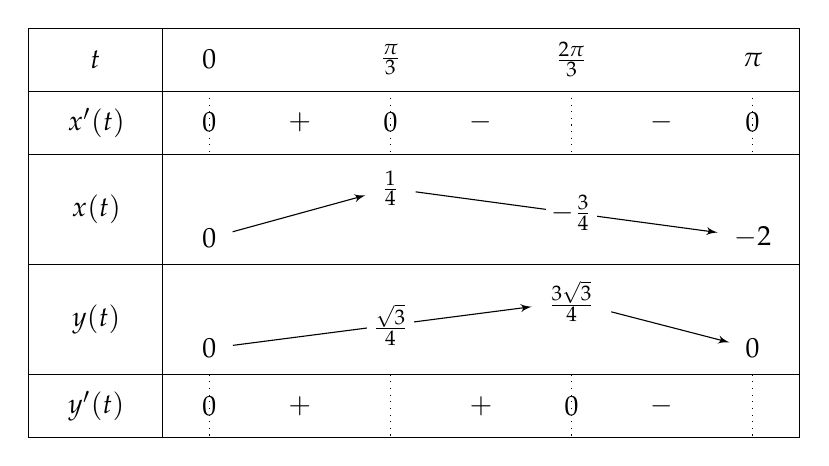
\begin{tikzpicture}
\tkzTabInit[lgt=1.7,espcl=2.3,deltacl=0.6]{$t$/0.8,$x'(t)$/0.8,$x(t)$/1.4,$y(t)$/1.4,$y'(t)$/0.8}{$0$,$\frac\pi3$,$\frac{2\pi}3$,$\pi$}
\tkzTabLine{z,+,z,-,t,-,z}
\tkzTabVar{-/$0$,+/$\frac14$,R/,-/$-2$}
\tkzTabIma{2}{4}{3}{$-\frac34$}
\tkzTabVar{-/$0$,R/,+/$\frac{3\sqrt3}4$,-/$0$}
\tkzTabIma{1}{3}{2}{$\frac{\sqrt3}4$}
\tkzTabLine{z,+,t,+,z,-,t}
\end{tikzpicture}
\end{center}
Tangente verticale en $\left(\frac14,\frac{\sqrt3}4\right)$ et en $(-2,0)$ ($f'(\pi)=(0,-2)$) ; horizontale en
$\left(-\frac34,\frac{3\sqrt3}4\right)$.

\q{4.} $f'(0)=\ve0$. Avec $1-\cos t=\frac{t^2}2+o(t^3)$ : $x=\frac{t^2}2+o(t^3)$, $y=\frac{t^2}2\cdot t+o(t^3)$, donc
$f(t)=t^2\left(\tfrac12,0\right)+t^3\left(0,\tfrac12\right)+o(t^3)$ : rebroussement de première espèce, tangente $(Ox)$, la courbe
arrivant du côté $x>0$. (À l'ordre 4, le terme $t^4\left(-\frac7{24},0\right)$ ne change rien : il est colinéaire
au premier.)

\q{5.} On place $O$ (pointe), les tangentes verticales et horizontale, on relie, puis on complète par symétrie d'axe $(Ox)$.
En polaire, $r=1-\cos\theta$ (\HP).
\begin{center}
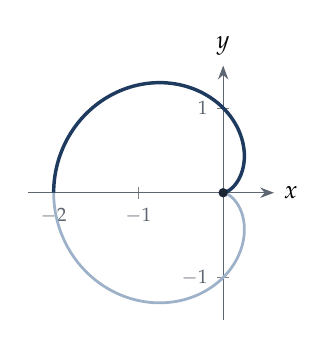
\begin{tikzpicture}
\begin{axis}[courbe,width=0.46\linewidth,xmin=-2.3,xmax=0.6,ymin=-1.5,ymax=1.5,xtick={-2,-1},ytick={-1,1}]
\addplot[reste,domain=-3.1416:0,samples=200]({(1-cos(x))*cos(x)},{(1-cos(x))*sin(x)});
\addplot[arcetude,domain=0:3.1416,samples=200]({(1-cos(x))*cos(x)},{(1-cos(x))*sin(x)});
\node[pt] at (axis cs:0,0) {};
\end{axis}
\end{tikzpicture}
\end{center}
\gain{$x'$ se factorise plus vite directement : $x'=-\sin t+2\cos t\sin t=\sin t(2\cos t-1)$. Choisir la factorisation la plus
courte, pourvu qu'elle donne le signe.}
\piege{en $t=\pi$, $x'=0$ mais $y'=-2\neq0$ : point régulier à tangente verticale, pas un point stationnaire.}
\retenir{$e^{ia}\pm e^{ib}=e^{i\frac{a+b}2}(\dots)$ : la factorisation par l'angle moitié est l'outil des dérivées
trigonométriques.}
\par\hfill\textcolor{BleuClair}{$\square$}\par
\soustitre{3}{La cubique de Descartes}{c:td-c8}
\choix{même structure que la lemniscate (exercice~17 du TD) : $t\mapsto\frac1t$ échange $x$ et $y$. Pour l'asymptote : méthode~2.4 du livre
}
\q{1.} $x(1/t)=\frac{1/t}{1+1/t^3}=\frac{t^2}{t^3+1}=y(t)$ et $y(1/t)=x(t)$ : symétrie par rapport à $\Delta:y=x$. Comme $t\mapsto\frac1t$
échange $]-1,1[\setminus\{0\}$ et $]-\infty,-1[\cup]1,+\infty[$, l'étude sur $]-1,1[$ suffit.

\q{2.} $x'(t)=\frac{1-2t^3}{(1+t^3)^2}$, $y'(t)=\frac{t(2-t^3)}{(1+t^3)^2}$. Sur $]-1,1[$ : $x'$ s'annule en $t_1=2^{-1/3}$, $y'$ en
$0$. Quand $t\to-1^+$, $x\to-\infty$, $y\to+\infty$. $M(0)=O$, tangente horizontale ; $M(t_1)=\left(\frac23 2^{-1/3},\frac23 2^{-2/3}\right)
\approx(0{,}53\,;0{,}42)$, tangente verticale ; $M(1)=\left(\frac12,\frac12\right)$, tangente perpendiculaire à $\Delta$.

\q{3.} $\frac yx=t\to-1$ et $y+x=\frac{t(1+t)}{1+t^3}=\frac t{1-t+t^2}\to-\frac13$ (simplification par $1+t$) : asymptote
$\mathcal D:y=-x-\frac13$. Position :
\[y+x+\frac13=\frac{3t+1-t+t^2}{3(t^2-t+1)}=\frac{(t+1)^2}{3(t^2-t+1)}>0 :\]
la courbe est \emph{au-dessus} de $\mathcal D$, des deux côtés.
\begin{center}
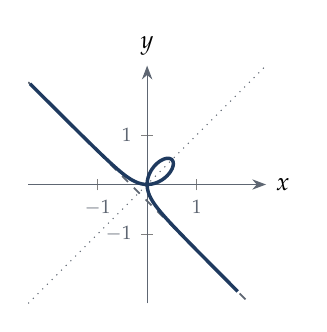
\begin{tikzpicture}
\begin{axis}[courbe,width=0.44\linewidth,xmin=-2.4,xmax=2.4,ymin=-2.4,ymax=2.4,xtick={-1,1},ytick={-1,1}]
\addplot[asy,domain=-2.4:2.4,samples=2]{-x-1/3};
\addplot[Gris,dotted,domain=-2.4:2.4,samples=2]{x};
\addplot[arcetude,domain=-0.86:40,samples=600]({x/(1+x^3)},{x^2/(1+x^3)});
\addplot[arcetude,domain=-40:-1.18,samples=300]({x/(1+x^3)},{x^2/(1+x^3)});
\end{axis}
\end{tikzpicture}
\end{center}
\gain{factoriser $1+t^3=(1+t)(1-t+t^2)$ dès le départ : la valeur interdite $-1$ et la simplification de $y+x$ apparaissent
aussitôt.}
\piege{conclure à l'asymptote avec $\frac yx\to-1$ seul : il faut $\lim(y+x)$.}
\retenir{position par rapport à une asymptote : mettre $y-(\alpha x+\beta)$ sur un dénominateur commun ; un carré au numérateur
signale que la courbe reste du même côté.}
\par\hfill\textcolor{BleuClair}{$\square$}\par
\soustitre{4}{Une famille de cubiques}{c:sel-c-2014}
\q{1.(a)} $x(-t)=-t^3+3t^2+9t=-(t^3-3t^2-9t)=-y(t)$ et de même $y(-t)=-x(t)$. Donc $M(-t)=\big(-y(t),-x(t)\big)$ : c'est l'image de $M(t)$ par $(x,y)\mapsto(-y,-x)$, la réflexion d'axe $\Delta:y=-x$. Comme $t\mapsto-t$ échange $\R_+$ et $\R_-$, on étudie la courbe pour $t\geq0$ et l'on complète par la symétrie d'axe $\Delta$.
\choix{le tableau du cours ne contient pas cette symétrie telle quelle : elle combine $t\mapsto-t$ et l'échange de $x$ et $y$. Toujours comparer $x(-t)$ à $\pm x(t)$ \emph{et} à $\pm y(t)$.}

\q{1.(b)} $x'(t)=3t^2+6t-9=3(t-1)(t+3)$ et $y'(t)=3t^2-6t-9=3(t-3)(t+1)$ : pas de zéro commun, tous les points sont réguliers.
\begin{center}
\renewcommand{\arraystretch}{1.25}
\begin{tabular}{c|ccccccc}
$t$ & $0$ & & $1$ & & $3$ & & $+\infty$\\\hline
$x$ & $0$ & $\searrow$ & $-5$ & $\nearrow$ & $27$ & $\nearrow$ & $+\infty$\\
$y$ & $0$ & $\searrow$ & $-11$ & $\searrow$ & $-27$ & $\nearrow$ & $+\infty$
\end{tabular}
\end{center}
Tangente verticale en $M(1)=(-5,-11)$ ($x'(1)=0$, $y'(1)=-12\neq0$) ; tangente horizontale en $M(3)=(27,-27)$ ($y'(3)=0$, $x'(3)=36\neq0$). En $t=0$, $f'(0)=(-9,-9)$ : la tangente en $O$ est la droite $y=x$.
\piege{« $x'=0$ donc tangente verticale » exige $y'\neq0$ au même point.}

\q{1.(c)} Pour $t\neq s$, on divise $x(t)-x(s)$ et $y(t)-y(s)$ par $t-s$ :
\[\frac{x(t)-x(s)}{t-s}=t^2+ts+s^2+3(t+s)-9,\qquad\frac{y(t)-y(s)}{t-s}=t^2+ts+s^2-3(t+s)-9.\]
Ces deux quantités sont nulles si et seulement si leur différence $6(t+s)$ et l'une d'elles le sont : $s=-t$, puis $t^2-9=0$. Le seul point double est $M(3)=M(-3)=(27,-27)$, situé sur $\Delta$. Les tangentes sont dirigées par $f'(3)=(36,0)$ et $f'(-3)=(0,36)$ : elles sont \emph{perpendiculaires}.
\choix{diviser par $t-s$ élimine la solution parasite $t=s$ ; on travaille ensuite avec des expressions symétriques en $t$ et $s$.}

\q{1.(d)} Quand $t\to+\infty$, $x$ et $y$ tendent vers $+\infty$, $\frac yx\to1$ et $y-x=-6t^2\to-\infty$ : branche parabolique de direction $y=x$.
\piege{$\lim\frac yx=1$ ne suffit pas : c'est $\lim(y-x)$ qui tranche entre asymptote et branche parabolique.}

\q{1.(e)} Pour $t\geq0$ : départ de $O$ vers le bas et la gauche (tangente $y=x$), tangente verticale en $(-5,-11)$, tangente horizontale au point double $(27,-27)$, puis branche parabolique vers le haut et la droite. On complète par la réflexion d'axe $y=-x$ ; la boucle est parcourue pour $t\in[-3,3]$.

\q{2.} $M(t)$ est stationnaire si et seulement si $3t^2+6t-a=0$ et $3t^2-6t-b=0$. La différence donne $12t=a-b$, la somme $6t^2=a+b$.
\emph{Condition nécessaire :} $t=\frac{a-b}{12}$ et $6\frac{(a-b)^2}{144}=a+b$, soit $(a-b)^2=24(a+b)$.
\emph{Réciproque :} si $(a-b)^2=24(a+b)$, on pose $t=\frac{a-b}{12}$ ; alors $3t^2=\frac{a+b}2$ et $6t=\frac{a-b}2$, d'où $x'(t)=\frac{a+b}2+\frac{a-b}2-a=0$ et $y'(t)=\frac{a+b}2-\frac{a-b}2-b=0$.
\retenir{un « si et seulement si » demande les deux sens ; la réciproque est souvent une vérification de deux lignes, à ne pas oublier.}
\par\hfill\textcolor{BleuClair}{$\square$}\par
\soustitre{5}{Problème de synthèse, type devoir surveillé}{c:ds-pb}
\choix{chaque question réinvestit une méthode du livre (factorisation des dérivées, développement en $t_0\neq0$, position globale, asymptotes, courbe asymptote, inflexion par factorisation de la vitesse). On note les valeurs interdites dès le début : $-3$ (borne) et $0$.}

\textbf{1.(a)} $x'(t)=-\frac4{t^2}+\frac1{t+3}=\frac{t^2-4t-12}{t^2(t+3)}=\frac{(t-6)(t+2)}{t^2(t+3)}$ et
$y'(t)=1-\frac4{t^2}=\frac{(t-2)(t+2)}{t^2}$. Comme $t^2>0$ et $t+3>0$, les signes se lisent sur les facteurs affines. Limites et
valeurs : $x\to-\infty$, $y\to-\frac{13}3$ quand $t\to-3$ ; $M(-2)=(-2,-4)$ ($\ln1=0$) ; $x,y\to-\infty$ quand $t\to0^-$ et
$+\infty$ quand $t\to0^+$ ; $M(2)=(2+\ln5,\,4)$ ; $M(6)=\left(\frac23+\ln9,\,\frac{20}3\right)$ ; $x,y\to+\infty$ quand $t\to+\infty$.
\begin{center}
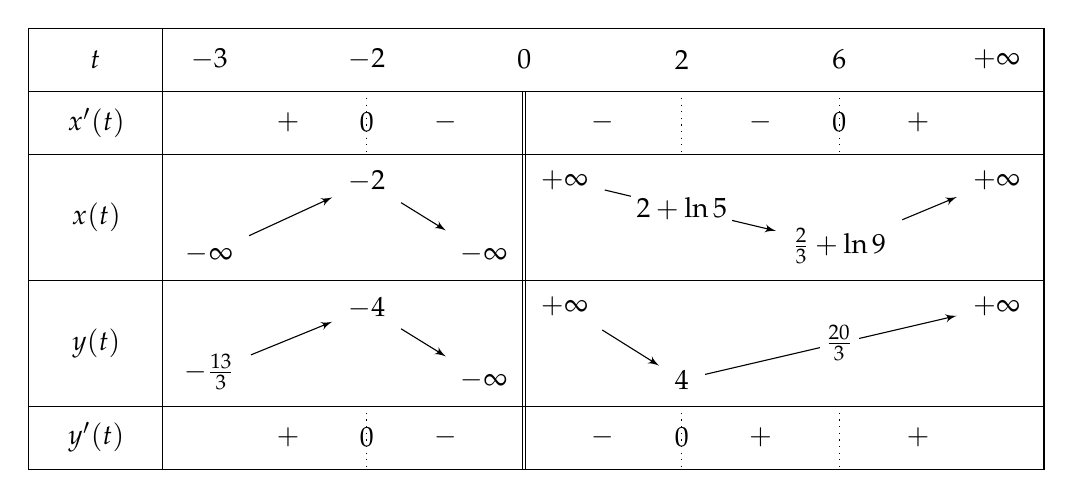
\begin{tikzpicture}
\tkzTabInit[lgt=1.7,espcl=2,deltacl=0.6]{$t$/0.8,$x'(t)$/0.8,$x(t)$/1.6,$y(t)$/1.6,$y'(t)$/0.8}{$-3$,$-2$,$0$,$2$,$6$,$+\infty$}
\tkzTabLine{,+,z,-,d,-,t,-,z,+,}
\tkzTabVar{-/$-\infty$,+/$-2$,-D+/$-\infty$/$+\infty$,R/,-/$\frac23+\ln9$,+/$+\infty$}
\tkzTabIma{3}{5}{4}{$2+\ln5$}
\tkzTabVar{-/$-\frac{13}3$,+/$-4$,-D+/$-\infty$/$+\infty$,-/$4$,R/,+/$+\infty$}
\tkzTabIma{4}{6}{5}{$\frac{20}3$}
\tkzTabLine{,+,z,-,d,-,z,+,t,+,}
\end{tikzpicture}
\end{center}

\textbf{(b)} Tangente verticale : $x'=0$ et $y'\neq0$, soit $t=6$ ($t=-2$ annule les deux) :
$A=M(6)=\left(\frac23+2\ln3,\frac{20}3\right)\approx(2{,}86\,;6{,}67)$. Tangente horizontale : $y'=0$, $x'\neq0$, soit $t=2$ :
$B=M(2)=(2+\ln5,4)\approx(3{,}61\,;4)$.

\textbf{(c)} Pour $t\notin\{-2,6\}$, $p(t)=\frac{y'(t)}{x'(t)}=\frac{(t-2)(t+2)}{t^2}\cdot\frac{t^2(t+3)}{(t-6)(t+2)}=\frac{(t-2)(t+3)}{t-6}$.
Alors $p(t)=m\iff t^2+t-6=m(t-6)\iff t^2+(1-m)t+6(m-1)=0$, de discriminant
$(1-m)^2-24(m-1)=(m-1)(m-25)$. Il est strictement négatif pour $1<m<25$ : aucune tangente n'a une pente dans $]1,25[$. Pour
$m=25$, la racine est double : $t=\frac{m-1}2=12$, qui est bien dans le domaine. D'où un unique point
$H=M(12)=\left(\frac13+\ln15,\frac{37}3\right)\approx(3{,}04\,;12{,}33)$.

\textbf{2.(a)} $\frac4{-2+h}=-\frac2{1-h/2}=-2-h-\frac{h^2}2-\frac{h^3}4+o(h^3)$ et $\ln(3+t)=\ln(1+h)=h-\frac{h^2}2+\frac{h^3}3+o(h^3)$.
D'où $x=-2-h^2+\frac{h^3}{12}+o(h^3)$, $y=-2+h+\frac4{-2+h}=-4-\frac{h^2}2-\frac{h^3}4+o(h^3)$ :
\[f(-2+h)=(-2,-4)+h^2\left(-1,-\tfrac12\right)+h^3\left(\tfrac1{12},-\tfrac14\right)+o(h^3).\]

\textbf{(b)} $\ve a=\left(-1,-\frac12\right)$ et $\ve b=\left(\frac1{12},-\frac14\right)$ ne sont pas colinéaires
($\det(\ve a,\ve b)=\frac14+\frac1{24}=\frac7{24}\neq0$) : $p=2$, $q=3$, $C$ est un point de \emph{rebroussement de première
espèce}. La tangente est dirigée par $\ve a$, ou par $(2,1)$ : $\det\big((x+2,y+4),(2,1)\big)=(x+2)-2(y+4)=0$, soit $x-2y=6$.

\textbf{(c)} Avec le développement : $\varphi(-2+h)=x-2y-6=-h^2+\frac{h^3}{12}+h^2+\frac{h^3}2+o(h^3)=\frac7{12}h^3+o(h^3)$.
La courbe traverse sa tangente en $C$ (rebroussement de première espèce) : elle est du côté $\varphi>0$, c'est-à-dire
\emph{au-dessous} de $T_C$ ($y<\frac{x-6}2$), pour $t$ un peu supérieur à $-2$, et au-dessus pour $t$ un peu inférieur.

\textbf{(d)} Méthode~2.5 du livre : $\varphi(t)=\ln(3+t)-2t-\frac4t-6$ et
\[\varphi'(t)=\frac1{t+3}-2+\frac4{t^2}=\frac{-2t^3-5t^2+4t+12}{t^2(t+3)}=-\frac{(t+2)^2(2t-3)}{t^2(t+3)}.\]
La racine double $-2$ était prévisible ($\varphi(-2)=\varphi'(-2)=0$ en un point de la tangente) et guide la factorisation.
Sur $]-3,0[$, $2t-3<0$ donc $\varphi'\geq0$ : $\varphi$ croît et s'annule en $-2$, d'où $\varphi<0$ sur $]-3,-2[$ et $\varphi>0$ sur
$]-2,0[$. Sur $]0,+\infty[$, $\varphi$ croît jusqu'en $\frac32$ puis décroît ; son maximum
$\varphi\left(\frac32\right)=\ln\frac92-\frac{35}3\approx-10{,}2$ est négatif : $\varphi<0$. Conclusion : $\mathcal C$ ne rencontre
$T_C$ qu'en $C$ ; elle est au-dessus de $T_C$ pour $t\in\,]-3,-2[\,\cup\,]0,+\infty[$ et au-dessous pour $t\in\,]-2,0[$, ce
qui prolonge l'étude locale.

\textbf{3.(a)} Quand $t\to0$, $x$ et $y$ sont infinis ; $\frac yx=\frac{t^2+4}{4+t\ln(3+t)}\to1$ et
$y-x=t-\ln(3+t)\to-\ln3$ : $\Delta_0:y=x-\ln3$ est asymptote. Position :
$y-x+\ln3=t-\ln\left(1+\frac t3\right)=\frac{2t}3+o(t)$ : au-dessus de $\Delta_0$ quand $t\to0^+$ (côté $x\to+\infty$),
au-dessous quand $t\to0^-$.

\textbf{(b)} Quand $t\to-3$, $x\to-\infty$ et $y\to-\frac{13}3$ : $\Delta':y=-\frac{13}3$ est asymptote horizontale. Comme $y$
est strictement croissante sur $]-3,-2]$, $y(t)>-\frac{13}3$ : la courbe est au-dessus de $\Delta'$.

\textbf{4.(a)} $x\sim\ln t$ et $y\sim t$, donc $\frac yx\to+\infty$ : branche parabolique de direction $(Oy)$.

\textbf{(b)} $e^{x(t)}=(3+t)\,e^{4/t}=(3+t)\left(1+\frac4t+\frac8{t^2}+O\!\left(\frac1{t^3}\right)\right)=t+7+\frac{20}t+O\!\left(\frac1{t^2}\right)$,
donc $\big(e^{x(t)}-7\big)-y(t)=\frac{16}t+O\!\left(\frac1{t^2}\right)\to0^+$. Le point $P_t=\big(x(t),e^{x(t)}-7\big)$ de
$\mathcal E$ vérifie $M(t)P_t\to0$ : $\mathcal E$ est asymptote, et la courbe est au-dessous.

\textbf{(c)} Le point de $y=e^x+c$ de même ordonnée est $Q_t=\big(\ln(y(t)-c),y(t)\big)$, et
$x(t)-\ln\big(y(t)-c\big)=\frac4t+\ln\frac{3+t}{t+\frac4t-c}\to0$ \emph{quel que soit} $c$. La distance horizontale ne
distingue aucune constante, alors que la distance verticale, $e^x+c-y\to7+c$, ne tend vers $0$ que pour $c=-7$. Pour une courbe
asymptote très pentue, on précise donc toujours quelle distance on utilise ; la plus exigeante est la distance verticale.

\textbf{5.(a)} $f'(t)=\lambda(t)\ve g(t)$ avec $\ve g(t)=\big(t-6,(t-2)(t+3)\big)=(t-6,t^2+t-6)$. Alors
$f''=\lambda'\ve g+\lambda\ve g'$ et, par bilinéarité, $\det(f',f'')=\lambda\lambda'\det(\ve g,\ve g)+\lambda^2\det(\ve g,\ve g')=\lambda^2\det(\ve g,\ve g')$.

\textbf{(b)} $\ve g'(t)=(1,2t+1)$ et $\det(\ve g,\ve g')=(t-6)(2t+1)-(t^2+t-6)=t^2-12t=t(t-12)$. En un point régulier
($t\neq-2$), $\lambda(t)\neq0$ : le seul candidat est $t=12$, et $\det(f',f'')$ change de signe en $12$ (racine simple, $\lambda^2>0$) :
$N=M(12)$ est l'unique point d'inflexion. C'est le point $H$ : d'après le \S2.4 ($p'=\frac{\det(f',f'')}{x'^2}$), la pente est extrémale en un
point d'inflexion à tangente non verticale. Ici $p$ décroît de $+\infty$ à $25$ sur $]6,12]$ puis croît : l'équation $p(t)=25$ a une
racine double en $12$.

\textbf{(c)} $T_N:y-\frac{37}3=25\left(x-\frac13-\ln15\right)$, soit $y=25x+12-25\ln15$.

\textbf{6.} On trace les asymptotes $\Delta_0$, $\Delta'$ et la courbe $\mathcal E$, on place $A$, $B$, $C$, $N$ avec leurs tangentes,
puis on suit le tableau : pour $t\in\,]-3,-2]$, la courbe vient de la gauche au-dessus de $\Delta'$ et monte jusqu'au
rebroussement $C$ ; elle repart vers le bas à gauche le long de $\Delta_0$ (au-dessous). Pour $t>0$, elle descend de l'infini le long
de $\Delta_0$ (au-dessus) jusqu'à $B$, remonte vers la gauche jusqu'à $A$, puis s'élève en traversant sa tangente en $N$ et longe
$\mathcal E$.
\begin{center}
\begin{tikzpicture}
\begin{axis}[courbe,width=0.86\linewidth,height=0.86\linewidth,axis equal image=false,xmin=-9,xmax=8,ymin=-10,ymax=14,
  xtick={-6,-2,2,6},ytick={-8,-4,4,8,12},restrict x to domain=-9:8,restrict y to domain=-10:14]
\addplot[asy,domain=-9:8,samples=2]{x-1.0986};
\addplot[asy,domain=-9:-1,samples=2]{-13/3};
\addplot[asy,domain=1.6:3.1,samples=60]{exp(x)-7};
\addplot[arcetude,domain=-2.99995:-0.42,samples=500]({4/x+ln(3+x)},{x+4/x});
\addplot[arcetude,domain=0.62:13.6,samples=500]({4/x+ln(3+x)},{x+4/x});
\addplot[tgte,domain=-4.5:0.5,samples=2]{(x-6)/2};
\addplot[tgte,samples=2] coordinates {(2.864,5.7) (2.864,7.6)};
\addplot[tgte,domain=2.9:4.3,samples=2]{4};
\addplot[tgte,domain=2.98:3.10,samples=2]{25*x+12-25*2.70805};
\node[pt] at (axis cs:-2,-4) {}; \node[font=\scriptsize,anchor=south east] at (axis cs:-2,-3.9) {$C$};
\node[pt] at (axis cs:2.864,6.667) {}; \node[font=\scriptsize,anchor=east] at (axis cs:2.8,6.667) {$A$};
\node[pt] at (axis cs:3.609,4) {}; \node[font=\scriptsize,anchor=north] at (axis cs:3.609,3.8) {$B$};
\node[pt,fill=Ocre] at (axis cs:3.041,12.333) {}; \node[font=\scriptsize,anchor=east] at (axis cs:2.95,12.333) {$N=H$};
\node[font=\scriptsize,Gris,anchor=west] at (axis cs:5.2,3.3) {$\Delta_0$};
\node[font=\scriptsize,Gris,anchor=south] at (axis cs:-7.5,-4.3) {$\Delta'$};
\node[font=\scriptsize,Gris,anchor=west] at (axis cs:3.12,14) {$\mathcal E$};
\end{axis}
\end{tikzpicture}
\end{center}
\retenir{le devoir enchaîne toujours les mêmes blocs : dérivées factorisées et tableau ; tangentes particulières (vérifier la
régularité) ; point stationnaire par développement en $t_0+h$ ; position locale puis globale ($\varphi$, racine double au point de
tangence) ; asymptotes à chaque valeur interdite et borne ; inflexion par factorisation de la vitesse ; dessin fidèle aux
positions.}
\par\hfill\textcolor{BleuClair}{$\square$}\par
\end{document}
